\documentclass[11pt]{beamer}
\usetheme{Goettingen}
\usepackage[utf8]{inputenc}
\usepackage{amsmath}
\usepackage{amsfonts}
\usepackage{amssymb}
\usepackage{graphicx}
\usepackage{hyperref}
\author{Alex Heilman}
\title{Point Group Equivariant Networks for Material Systems}
\subtitle{Thesis Proposal}
%\setbeamercovered{transparent} 
%\setbeamertemplate{navigation symbols}{} 
%\logo{} 
%\institute{} 
%\date{} 
%\subject{} 



\newenvironment{boxed2}
    {\begin{center}
    \begin{tabular}{|p{0.95\textwidth}|}
    \hline\\
    }
    { 
    \\\\\hline
    \end{tabular} 
    \end{center}
    }


\begin{document}

\begin{frame}
\titlepage
\end{frame}

\begin{frame}{Overview}
	$\bullet$ Graph Neural Networks for Materials Science
	
	\vspace{0.5cm}
	
	$\bullet$ Hypergraph representations
	
	\vspace{0.5cm}
	
	$\bullet$ Importance of Equivariance
	
	\vspace{0.5cm}
	
	$\bullet$ $O(3)$ Equivariance \& Tensor Predictions
	
	\vspace{0.5cm}
	
	$\bullet$ Why we should use material symmetry groups!
\end{frame}

%\begin{frame}
%\tableofcontents
%\end{frame}


\begin{frame}{Why Neural Networks?}
	Physics assumes there exists a map between configurations and properties of physical systems: 
	$$
	\lbrace\vec{r}_i \rbrace \xrightarrow[\text{Nature}]{}
	\lbrace\vec{r}_i' \rbrace
	$$
	Neural network techniques assume maps between abstract input and output spaces exist:
	$$
	X
	\xrightarrow[\text{Neural Network}]{}
	Y
	$$
	and that these may be expressed in a basis of adequately large neural networks.
	
	\vspace{0.5cm}
	
	\begin{center}
		But how do we apply this to material systems?
	\end{center}
	
\end{frame}

\begin{frame}{Machine Learning on Crystal Systems}
To perform predictive tasks for material systems, such as crystalline structures, we essentially need two things:

\medskip

$\bullet$ A way to represent the material system mathematically

\medskip

$\bullet$ A trainable predictive model or set of functions which takes, as input, the material system's representation (as well as a large set of data)
\end{frame}


\section{Graph Neural Networks}
\begin{frame}{Usual Crystal Graph Construction \small(a la CGCNN)}

The usual technique is to represent crystalline systems as graphs (nodes and edges), with atomic features associated with nodes and geometric features associated with edges

\medskip

\begin{center}

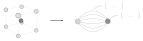
\includegraphics[scale=0.7]{crystalgraph.pdf}

\end{center}
\end{frame}

\begin{frame}{Crystal Graphs cont. I}

$\bullet$ Edges are determined by distance cutoff (4 Ang.) and maximum number of neighbors (12)

\begin{center}
\includegraphics[scale=0.45]{ex_bondcriteria.pdf}
\end{center}
\end{frame}

\begin{frame}{Crystal Graphs cont. II}
Edge attributes then are a Gaussian distance expansion

\begin{center}
\includegraphics[scale=0.33]{bond_feat.pdf}
\end{center}
\end{frame}

\begin{frame}{Message Passing on Graphs}
Now, we need to update these features through some trainable function that acts on graph representations.


\medskip

This is most generally accomplished by a message passing network applied to graph representations.
\begin{gather*}
m_i^{t+1}=\sum_{n_j\in \mathcal{N}(i)} M_t(n_i^{t},e_{ij},n_j^t )\\
\\
n_i^{t+1}=U_t(n_i^t,m_i^{t+1})\\
\end{gather*}
Here, each node $n$ from layer $t$ to $t+1$ is updated according to an update function $U$, which takes as input messages formed from each pair of nodes containing the node to be updated.
\end{frame}
\begin{frame}{Graph Neural Network}
	Add schematic with pooling
\end{frame}

\begin{frame}{Graph Limitations}
Problem: Our underlying representation encodes only distances between atoms!

\begin{center}

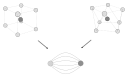
\includegraphics[scale=0.7]{crystalgraph_cntex.pdf}

\end{center}

So, as a rough example, the above two crystalline structures would have the same representations!
\end{frame} 

\subsection{Crystal Hypergraphs}
\begin{frame}{Solution: Hypergraphs!}
Hypergraphs allow us to have edges containing more than (or less than) two nodes.

\begin{center}
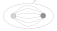
\includegraphics[scale=0.7]{hyperedge_ex.pdf}
\end{center}

This gives us a natural way to encode features with higher order structure, where hypergraph nodes still represent atoms of underlying crystal structure.

\vspace{.5cm}

Can treat all different order structures in crystals on equal footing: each has a corresponding hyperedge with a feature
\end{frame}


\begin{frame}{Local Environments as Hyperedges}


Considering our previous problem, we can now encode this lost geometrical information in larger hyperedges:

\medskip

\hspace{1cm}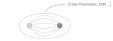
\includegraphics[scale=0.7]{motiflevel_ex.pdf}

\medskip

This geometrical information can be encoded quantitatively with continuous symmetry measures, local structure order parameters, etc., depending on task


\end{frame}


\begin{frame}{Extending Message Passing to Hypergraphs}

Now, we need a suitable convolutional structure that applies to hypergraphs...

\medskip

In this case, the neighborhood of nodes relevant to each message are now a set (instead of the single neighboring node feature of classic MPNNs)

\begin{gather*}
m_i^{t+1}=\sum_{h_j\ni x_i} M_t(n_i^{t},\underbrace{h_j^{t},\lbrace  n_w^t \vert n_w \in h_j }_{e_{ij},n_j}\rbrace)\\
\\
n_i^{t+1}=U_t(n_i^t,m_i^{t+1})\\
\end{gather*}
\end{frame}



\begin{frame}{Hypergraph Convolution}
To deal with the variable sized neighborhoods of features, we simply aggregate the neighborhood features in the message passing phase, so that we essentially have the following form of convolution:
\begin{align*}
x_i \rightarrow x_i &+ f_b(x_i\oplus e_{ij} \oplus \text{AGG}(\lbrace x_i, x_j\rbrace))\\
&+ f_m(x_i\oplus m_{j} \oplus \text{AGG}(\lbrace  n_w^t \vert n_w \in m_j \rbrace))
\end{align*}
where we only consider pair-wise and local environment hyperedges above (with other order structures, such as triplet and unit cell level hyperedges also fitting into this framework). This allows us to effectively capture higher-order geometric features in an invariant manner!

\vspace{0.6cm}

\begin{center}
	But what if we care about about coordinate-system dependent quantities?
\end{center}

\end{frame}

\section{$O(3)$-Equivariant Networks}

\begin{frame}{Equivariant Functions}
	An equivariant function $f:X\rightarrow Y$, where $X,Y$ are vector spaces, is one that 'commutes' with a group's actions, satisfying:
	$$
	f\Big(\mathcal{D}^X(g)x\Big)=\mathcal{D}^Y(g)f(x)
	$$
	Tensor products are equivariant with respect to their argument vector spaces.
	
	Equivariance is always with respect to some group of transformations!
\end{frame}
\begin{frame}{Why Equivariant Functions?}
	\begin{center}
		Physical processes respect coordinate system rotations $R$:
		$$
		\lbrace R\vec{r}_i \rbrace \xrightarrow[\text{Nature}]{}
		\lbrace R\vec{r}_i' \rbrace
		$$
		In general, neural networks do not:
		$$
		RX
		\xrightarrow[\text{Neural Network}]{} \ \ 
		?
		$$
		
		So what do we want?
		
	\end{center}
\end{frame}
\begin{frame}{Equivariant Networks}
	\begin{center}
		We want equivariant networks for physics!
		
		$$
		RX
		\xrightarrow[\text{Neural Network}]{\text{Equivariant}} RY
		$$
		
		\vspace{0.6cm}
		
	\end{center}
	
	In equivariant networks, we consider feature vectors in basis of representation space as:
	$$
	v^{\alpha}_i
	$$
	with indexes $\alpha$ denoting the irrep it transforms as, and $i$ denoting the dimension of irrep space $\alpha$.
	
	
\end{frame}
\begin{frame}{Equivariant Networks (cont.)}
	Compositions of equivariant functions are equivariant \cite{tacovariant}. We consider building blocks:{\small
		\begin{itemize}
			
			\item Self-interaction:
			$$
			v'_{nc} = W^i_c v_{ni}
			$$
			\item Non-linear functions along channels  (for trivial irrep $\alpha=1$):
			$$
			v'_{nc}=f(v_{nc}+b_{nc})
			$$
			\item Group correlation with filters \cite{cohen_equivariant}:
			$$
			[F\star v](g)=\sum_{h\in G}\sum_c F_c(h)v_c(g^{-1}h)
			$$
			\item Tensor products with filters \cite{tensorfieldnetworks, e3nn}:
			$$
			(v'_{nc})^{\gamma}_{n} = \sum_{ij}U_{\alpha i \beta j}^{\gamma n}\big(F_{j}^{\beta}\otimes V^{\alpha}_i \big) 
			$$
			\item Pooling over nodes or channels:
			$$
			v_c = \sum_n v_{nc}
			$$
	\end{itemize}}
\end{frame}
\begin{frame}{$SO(3)$ Properties}
	Most modern equivariant networks are specifically $SO(3)$-Equivariant.
	
	\vspace{0.5cm}
	
	\begin{itemize}
		\item Inifinite order $\rightarrow$ infinite irreps
		\item Irreps are Wigner $\mathcal{D}^{\ell}$ matrices
		\item Natural basis set $Y^{\ell}_m$ of dimension $d_{\ell}=2\ell+1$
	\end{itemize}
	
	\vspace{0.5cm}
	
	Many models are further referred to as $E(3)$-equivariant for the Euclidean group (add parity and translation invariance).
\end{frame}

\begin{frame}{\textit{Tensor Field Networks}}
	Tensor field networks \cite{tfn} use SO(3) equivariant convolution:{\small
		$$
		\big(v^{L+1}_{nc}\big) ^{\ell}_{m}=\big(v^{L}_{nc}\big)^{\ell}_m+\sum_{b\in \mathcal{N}(n)}\sum_{\ell_f m_f , \ell_i m_i}^{\ell_{\text{max}} m_{\text{max}}}c_{\ell_fm_f\ell_im_i}^{\ell m}\big(F^{L}_c(r_{nb})\big)^{\ell_f}_{m_f}\big(v_{bc}^L \big)^{\ell_i}_{m_i}
		$$}
	\begin{itemize}
		\item $v_{nc}^{L}$: Node feature of node $n$, channel $c$, layer $L$
		\item $c_{\ell_fm_f\ell_im_i}^{\ell_om_o}$: Clebsch-Gordan coefficients
		\item $F_c^L$: Filter function (trainable)
		\item $r_{nb}$: Radius between nodes $n$ and neighbor $b\in \mathcal{N}(n)$
	\end{itemize}
	
	\vspace{.7cm}
	
	$F$ is generally a neural network; $r$ is often expanded with some radial basis function (RBF): Gaussian, Bessel, etc.
\end{frame}

\begin{frame}{$SO(3)$-Equivariant Features}
	Remember that node (and edge) features now have additional indices $\ell$ and $m$!
	$$
	\big(v^{L+1}_{nc}\big) ^{\ell}_{m}
	$$	
	
	This allows us to keep track of which components transform like which irreps of $SO(3)$.
	
	\vspace{0.6cm}
	
	\begin{center}
	But what can we do with this?
	\end{center}
\end{frame}

\subsection{Tensor Prediction}


\begin{frame}{$J_z$ Basis}
	Recall $\ell=1$ spherical harmonics (with Racah normalization):
	\begin{align*}
		Y_1^{+1} &= -\frac{1}{\sqrt{2}}(x+iy)=\frac{1}{\sqrt{2}}\sin \phi e^{i\theta}\\
		Y_1^{0}\ \ &= z = \cos \phi\\
		Y_1^{-1} &= -\frac{1}{\sqrt{2}}(x-iy)=\frac{1}{\sqrt{2}}\sin \phi e^{-i\theta}
	\end{align*}
	\begin{center}
		So, define $J_z$ basis:
		$$
		\begin{bmatrix}
			a_+ \\
			a_0 \\
			a_-
		\end{bmatrix}=\begin{bmatrix}
			-\frac{1}{\sqrt{2}} & -\frac{i}{\sqrt{2}} & 0\\
			0 & 0 & 1\\
			-\frac{1}{\sqrt{2}} & +\frac{i}{\sqrt{2}} & 0\\
		\end{bmatrix}\begin{bmatrix}
			x \\
			y \\
			z
		\end{bmatrix}
		$$
		so that $\hat{n}=a_+ Y_1^1 + a_0 Y_1^0 + a_- Y_1^{-1}$
	\end{center}
\end{frame}
\begin{frame}{Clebsch-Gordon Expansion}
	Build larger spherical harmonic tensors with CG expansion:
	$$
	Y_{\ell_1}^{m_1}\otimes Y_{\ell_2}^{m_2} = \sum_{L=-|\ell_1-\ell_2|}^{\ell_1+\ell_2}\sum_{M=-L}^{L}c_{\ell_1 0 \ell_2 0}^{L0}c_{\ell_1 m_1 \ell_2 m_2}^{LM}Y_{L}^M
	$$
	where $Y_{L}$ represents a $2L+1$ dimensional symmetric tensor space of rank $L$. 
	
	This serves as a relation between symmetric tensor's $J_z$ basis components and higher order spherical harmonic tensors. 
	
	$$ 
	T^{(n)} = a_{\underbrace{\alpha\beta...}_n}\big(Y_1^\alpha \otimes Y_1^\beta\otimes ... \big)\ \  \Rightarrow\ \  y_\ell^m Y_L^M
	$$
	
	\begin{center}
		But, what about asymmetric tensors?
	\end{center}
\end{frame}
\begin{frame}{$SO(3)$ Invariant Tensor Subspaces}
	We can always reduce an arbitrary tensor $T$ that transforms under a transformation as:
	$$
	T_{x_1x_2...x_n}\rightarrow T_{x'_1x'_2...x_n'}=R_{x_1'}^{x_1} R_{x_2'}^{x_2} R_{x_3'}^{x_3}T_{x_1x_2...x_n},
	$$
	into a set of irreducible (but not necessarily unique) symmetric, $SO(3)$ invariant subtensors:
	$$
	\lbrace h^{(\ell)}\rbrace \rightarrow \lbrace h'^{(\ell)}\rbrace = \lbrace \mathcal{D}^{\ell}(R) h^{(\ell)}\rbrace
	$$
	
	This decomposition can be constructed by consecutive decomposition with respect to $GL$ and then $O$ and $SL$
	$$
	SO= SL\cap O \subset GL
	$$
\end{frame}

\begin{frame}{$SO(3)$ Invariants Ex.: Rank 2}
Consider a rank-two tensor $E_{ij}$:

Decompose into symmetric $S$
$$
S_{ij}=\frac{1}{2}(E_{ij}+E_{ji})
$$
Then take trace $t = g_{ij}S_{ij}$ and residue $R=S-tg$.

And, antisymmetric $A$:
$$
A_{ij}=\frac{1}{2}(E_{ij}-E_{ji})
$$
\end{frame}




\begin{frame}{Tensor Prediction}
	Add schematic
\end{frame}


\begin{frame}{Tensor Prediction (cont.)}
	Add results
\end{frame}


\begin{frame}{Tensor Prediction with $SO(3)$-Networks}
	$\bullet$ We can read off the output of $SO(3)$-networks as tensor components 
	
	\vspace{0.3cm}
	
	$\bullet$ These naturally respect coordinate transformations acting on the input space!
	
	\vspace{0.3cm}
	
	$\bullet$ Can learn, but doesn't restrict to symmetry of crystals...
	
	\vspace{0.6cm}
	
	\begin{center}
		Can we get more out of symmetry considerations?
	\end{center}
\end{frame}

\section{Material Symmetry}
\begin{frame}{Material Symmetries}
	Add point group schematic
\end{frame}



\begin{frame}{Point Group Properties}
	Groups of operations that leave at least one point fixed and are compatible with a Bravais lattice.
	
	\vspace{0.3cm}
	
	Point groups (in 3D) have following properties:
	\begin{itemize}
		\item 32 crystallographic point groups in 3D
		\item Finite number of irreps for each
		\item All irreps of point groups are of dimension $d_{\alpha}=1,2,3$
		\item All allow a (often reducible) 3D representation
		\item Decompositions with $c_{\alpha\beta\gamma}=0,1,2$
	\end{itemize}
	
	{\small
		(Point group representations may be used to generate induced representations of space groups)}
\end{frame}

\begin{frame}{Site-symmetry Equivariant Networks}
	\begin{center}
		Index vectors by $\alpha ,i$  from site-symmetry group instead!
	\end{center}
	{\small
		$$
		\big(v^{L+1}_{nc}\big) ^{\ell}_{m}=\big(v^{L}_{nc}\big)^{\gamma}_n+\sum_{b\in \mathcal{N}(n)}\sum_{\alpha i, \beta j}U_{\alpha i \beta j}^{\gamma n}\big(F^{L}_c(r_{nb})\big)^{\beta }_{j}\big(v_{bc}^L \big)^{\alpha}_{i}
		$$}
	
	\begin{itemize}
		\item Natural cutoff (finite summation over $\alpha,\beta$)
		\item Natural readout for symmetric properties ($\gamma=1$)
		\item Accounts for all physical symmetry but not more
	\end{itemize}
	
\end{frame}


\begin{frame}{Coupling Coefficients}
	Coupling coefficients for point groups can be computed from irreps with
	Dirl's Formula \cite{dirl1979}:\footnotesize
	$$
	(U^{\gamma n}_{\alpha i \beta j})^m = \sqrt{\frac{d_{\gamma}}{N_{G}}}\Big[\sum_{g\in G}\Gamma^{\alpha}_{qq}(g)\Gamma^{\beta}_{ss}(g)\Gamma^{\gamma \dagger}_{aa}(g)\Big]^{-\frac{1}{2}}\cdot \sum_{g\in G}\Gamma^{\alpha}_{iq}(g)\Gamma^{\beta}_{js}(g)\Gamma^{\gamma\dagger}_{na}(g)
	$$
	With these models  we can predict:
	
	\vspace{0.3cm}
	
	$\bullet$ Scalar quantities that are invariant under material symmetry group (not just spherically symmetric)
	
	\vspace{0.3cm}
	
	$\bullet$ Tensor quantities that respect material symmetry
	
	\vspace{0.3cm}
	
	$\bullet$ Symmetry-adapted Hamiltonian elements
\end{frame}



\begin{frame}{Hamiltonian Group}
	We define the operator $\hat{O}_G$ to be a representation of a group $G$ that acts on $H$'s input space $\vec{r}$ as:
	$$
	\hat{O}_G(g)\hat{H}(\vec{r}) = \hat{H}(g^{-1}\vec{r})
	$$
	The "group of the Hamiltonian" is the largest group of the form above that commutes with the Hamiltonian.
	$$
	[\hat{H},\hat{O}(g)] = 0 \quad \quad \forall g \in G
	$$
	In such a case, the operators must have a simultaneous set of eigenvectors $\psi^{k}_{\alpha}$ that span the space of functions:
	
	$$
	f(\vec{r})=\sum_{k,\alpha}c_{k}^{\alpha}\psi^{k}_{\alpha} =\sum_{k,\alpha}f^k_{\alpha}(\vec{r})
	$$
	
	\medskip
	
	We have some freedom in choice of this set of basis functions on which the linear operators of the representations act.
\end{frame}
\begin{frame}{Hydrogen Orbitals}
	The Hydrogen Hamiltonian $\hat{H}_H(\vec{r})$ for a non-relativistic electron has separable eigenfunctions:
	$$
	\psi_i(\vec{r})=R_i(r)\Omega_i(\theta,\phi)
	$$
	Furthermore, $\hat{H}_H$ commutes with $SO(3)$ so these must be simultaneous with $SO(3)$:
	{\small
		$$
		[\hat{H},\hat{O}(g)] = 0 \quad \forall g \in SO(3) \quad \Rightarrow \quad \psi_{nm}^{\ell}(\vec{r})=R_{n}^{\ell}(r)Y^{\ell}_{m}(\theta,\phi)
		$$
		(where $R$ is also indexed by $\ell$ due to an 'accidental' symmetry) }
	
	\vspace{0.4cm}
	
	\begin{itemize}
		\item  $\theta,\phi$ dependence determined by group theory
		\item  $r$ dependence determined by specific form of $\hat{H}_H$
	\end{itemize}
\end{frame}
\begin{frame}{Tight-Binding Approximations}
	In simplest form, consider H-like orbitals $\vert \psi_{nmp}^{\ell}\rangle$ localized at points $p$ as basis for many particle system defined by $\hat{H}$ so:
	$$
	\hat{H}_{nmp\ell,jkhl}=\langle \psi_{jkh}^l\vert\hat{H}\vert\psi_{nmp}^{\ell}\rangle
	$$
	Now, we can incorporate point group symmetry of crystal and molecular sites by directly learning features associated with basis functions that transform as irreducible representations.
\end{frame}
\begin{frame}{Where to start? ($O_h$)}

	
	$\bullet$ The largest crystalline point group is $O_h$ (Most restriction on $SO(3)$)
	
	\vspace{0.3cm}
	
	$\bullet$ Materials Project \cite{matproj} contains 15,268 materials with this symmetry.
	
	\vspace{0.3cm}
	
	$\bullet$ Implement working concept model for $O_h$ systems that predicts invariant quantities
	
	\end{frame}


	\begin{frame}{References}
	
	\printbibliography
	
	\end{frame}


\end{document}